\documentclass[conference]{IEEEtran}
\IEEEoverridecommandlockouts
\usepackage{cite}
\usepackage{amsmath,amssymb,amsfonts}
\usepackage{graphicx}
\usepackage{textcomp}
\usepackage{xcolor}
\usepackage{booktabs}
\usepackage{tabularx}
\usepackage{multirow}
\usepackage{array}
\usepackage{threeparttable}
\usepackage{stfloats}
\usepackage{url}
\usepackage{tikz}
\usetikzlibrary{positioning,arrows.meta,fit,shapes.geometric}

\graphicspath{{../results/}}
\renewcommand{\ttdefault}{cmtt}
\newcommand{\km}{\,km}
\newcommand{\m}{\,m}

\begin{document}

\title{Auditing the RTE Compliance Gap: Network-Based Geospatial Analysis of Walking Access to Government Schools in Bengaluru's Formal and Informal Settlements}

\author{\IEEEauthorblockN{Kaveri Sharma}
\IEEEauthorblockA{\textit{Dept. of Computer Science Engg.} \\
\textit{PES University}\\
Bengaluru, India \\
kaveri05sharma@gmail.com}
\and
\IEEEauthorblockN{Vedika Chhabra}
\IEEEauthorblockA{\textit{Dept. of Computer Science Engg.} \\
\textit{PES University}\\
Bengaluru, India \\
vedikac11@gmail.com}
\and
\IEEEauthorblockN{Jahnvi R}
\IEEEauthorblockA{\textit{Dept. of Computer Science Engg.} \\
\textit{PES University}\\
Bengaluru, India \\
jahnvi04@gmail.com}
\and
\IEEEauthorblockN{Manasa Ranganath}
\IEEEauthorblockA{\textit{Dept. of Computer Science Engg.} \\
\textit{PES University}\\
Bengaluru, India \\
manasaranganath06@gmail.com}
\and
\IEEEauthorblockN{Komal Kumari}
\IEEEauthorblockA{\textit{Dept. of Computer Science Engg.} \\
\textit{PES University}\\
Bengaluru, India \\
jaiswalkomal048@gmail.com}
\and
\IEEEauthorblockN{Dr. Divyashree N}
\IEEEauthorblockA{\textit{Associate Professor} \\
\textit{PES University}\\
Bengaluru, India \\
divyashreen@pes.edu}
}

\maketitle

\begin{abstract}
India's Right to Education (RTE) rules promise every child a government primary school within a 1\km{} walk, yet compliance is audited with outdated habitation lists and straight-line buffers. We present an open, reproducible pipeline that audits this mandate on the real street network. Sentinel-2 imagery and a Random Forest delineate built-up morphology; an OpenStreetMap pedestrian graph (186,595 nodes) and a single multi-source shortest-path search partition Bengaluru into network catchments of government schools; and WorldPop 2020 population weights the results for all 509 Karnataka Slum Development Board (KSDB) slums. With a curated set of 111 government schools, only 17.3\% of 1,000 sampled locations and 20.1\% of 226,753 slum residents lie within a 1\km{} walk. Straight-line audits overstate compliance: 48.2\% of locations that look compliant by straight line are not compliant on foot. Non-notified slums are significantly worse served than notified ones (population-weighted 2.40 vs.\ 1.71\km{}, $p<10^{-5}$), and ten schools are the nearest government option for 71.5\% of slum residents. The difference between planned and informal areas is small and sensitive to how government schools are identified. Because OpenStreetMap under-records government schools, these figures are best read as lower bounds on access.
\end{abstract}

\begin{IEEEkeywords}
Right to Education, spatial accessibility, informal settlements, OpenStreetMap, OSMnx, network analysis, Dijkstra, Sentinel-2, Random Forest, WorldPop, Bengaluru.
\end{IEEEkeywords}

%=====================================================================
\section{Introduction}
%=====================================================================
Bengaluru grew to 8.44 million residents within municipal (BBMP) limits by 2011 \cite{census2011}, and much of its later growth has been unplanned and peripheral. Informal settlements produced by such growth often remain outside the planning record for years \cite{unhabitat2003}; of the 509 slum polygons published by the KSDB, 317 are \emph{non-notified}, i.e., recognised spatially but without the legal status that triggers service provision.

The RTE Act, 2009 \cite{rte2009}, and Rule~6 of the Central RTE Rules, 2010 \cite{rterules2010}, define the neighbourhood of a primary school (Classes I--V) as a 1\km{} walk and of an upper-primary school (Classes VI--VIII) as 3\km{}. Audits based on habitation lists cannot see settlements missing from the planning frame, and straight-line radii ignore the street network: a school 600\m{} away across a railway or an uncrossable arterial may be a 2\km{} walk. We call this the \emph{crow-flies fallacy}. Open data now allow a better audit: Sentinel-2 provides free 10\m{} imagery \cite{drusch2012}, Google Earth Engine (GEE) makes city-scale classification tractable \cite{gorelick2017}, OpenStreetMap (OSM) supplies a routable network \cite{boeing2017}, and WorldPop provides 100\m{} population grids \cite{tatem2017}.

\subsection{Contributions}
This paper makes four contributions:
\begin{enumerate}
\item An open, reproducible pipeline (Map $\rightarrow$ Detect $\rightarrow$ Measure $\rightarrow$ Weigh) that audits RTE walking-distance compliance from Sentinel-2, OSM, the KSDB register and WorldPop (Section~\ref{sec:method}).
\item An application of network Voronoi partitioning \cite{erwig2000,okabe2008} to RTE catchments, giving for every street node both the walking distance to and the identity of the nearest government school, and hence population-weighted catchment loads.
\item Evidence from real data that straight-line buffers roughly double apparent compliance (Section~\ref{sec:crowflies}), and that non-notified slums and peripheral zones are least served (Section~\ref{sec:slums}).
\item A transparent treatment of data-quality threats, including a sensitivity analysis on how ``government schools'' are identified in OSM (Sections~\ref{sec:data} and~\ref{sec:validity}).
\end{enumerate}

%=====================================================================
\section{Literature Survey}\label{sec:lit}
%=====================================================================
Slum mapping from space relies chiefly on texture and morphology in very-high-resolution (VHR) imagery \cite{kuffer2016,kohli2012}, and the scarcity of reliable ground truth is a persistent obstacle \cite{mahabir2018}. Grey-Level Co-occurrence Matrix (GLCM) texture \cite{haralick1973} explains much intra-urban variation in poverty \cite{duque2015}, and slum segmentation from 10\m{} Sentinel-2 data is feasible but markedly less accurate than from VHR data \cite{wurm2019}. Random Forests \cite{breiman2001} dominate operational remote-sensing classification \cite{belgiu2016}, typically with the NDVI \cite{tucker1979} and NDBI \cite{zha2003} indices as features.

Conclusions about the spatial equity of public facilities depend strongly on the accessibility measure used \cite{talen1998}; the two-step floating catchment area (2SFCA) method \cite{luo2003,radke2000} adds supply capacity when it is known. Network distances are computed on OSM graphs with OSMnx \cite{boeing2017} and NetworkX \cite{hagberg2008} using Dijkstra's algorithm \cite{dijkstra1959}, and nearest-facility catchments on a network form a network Voronoi diagram \cite{erwig2000,okabe2008}. OSM road networks are largely complete in large cities \cite{haklay2010,barrington2017}, but points of interest and their attributes, such as school ownership, are far less so.

Private schooling has grown rapidly in India \cite{kingdon2020,muralidharan2015}, so distance to a \emph{government} school measures the reach of the free option rather than access to any school. As Table~\ref{tab:lit} shows, slum-mapping studies stop at detection and accessibility studies assume a complete population frame. To our knowledge, no published study for an Indian city combines open satellite classification, the official slum register, gridded population and street-network routing to audit the RTE walking-distance mandate.

\begin{table*}[!t]
\centering
\caption{Comparison of Related Work}
\label{tab:lit}
\footnotesize
\begin{tabularx}{\textwidth}{@{}p{1.6cm}p{3.0cm}p{3.1cm}p{3.1cm}X@{}}
\toprule
\textbf{Study} & \textbf{Focus} & \textbf{Data} & \textbf{Method} & \textbf{Gap relative to this work} \\
\midrule
Kuffer \cite{kuffer2016} & Review of slum mapping & VHR, medium-resolution imagery & Texture, OBIA, ML & Detection only; no service access \\
Kohli \cite{kohli2012} & Slum ontology & VHR imagery & Rule-based ontology & No routing or population weighting \\
Duque \cite{duque2015} & Intra-urban poverty & VHR land cover & Texture metrics, regression & Poverty proxy, not service access \\
Wurm \cite{wurm2019} & Slum segmentation, Mumbai & QuickBird, Sentinel-2 & FCN transfer learning & No link to public services \\
Talen \cite{talen1998} & Equity of playgrounds & Facility points, census & Several accessibility measures & Census frame misses informal areas \\
Luo \cite{luo2003} & Health-care access & Facilities, census tracts & 2SFCA & Requires reliable capacity data \\
Boeing \cite{boeing2017} & Street-network tooling & OSM & Graph analytics & General tool; no application to RTE \\
\textbf{This work} & RTE compliance audit & Sentinel-2, OSM, KSDB, WorldPop & RF + network Voronoi catchments & --- \\
\bottomrule
\end{tabularx}
\end{table*}

%=====================================================================
\section{Study Area and Data}\label{sec:data}
%=====================================================================
\subsection{Study Area}
The study area is Bengaluru, Karnataka. Network routing and school features cover the OSM administrative boundary of the city. Satellite classification covers a 15\km{} radius around the city centre (12.9716$^\circ$N, 77.5946$^\circ$E). Fig.~\ref{fig:study} shows the distribution of KSDB slum polygons, the classified sample locations, and the curated government schools.

\begin{figure}[!t]
\centering
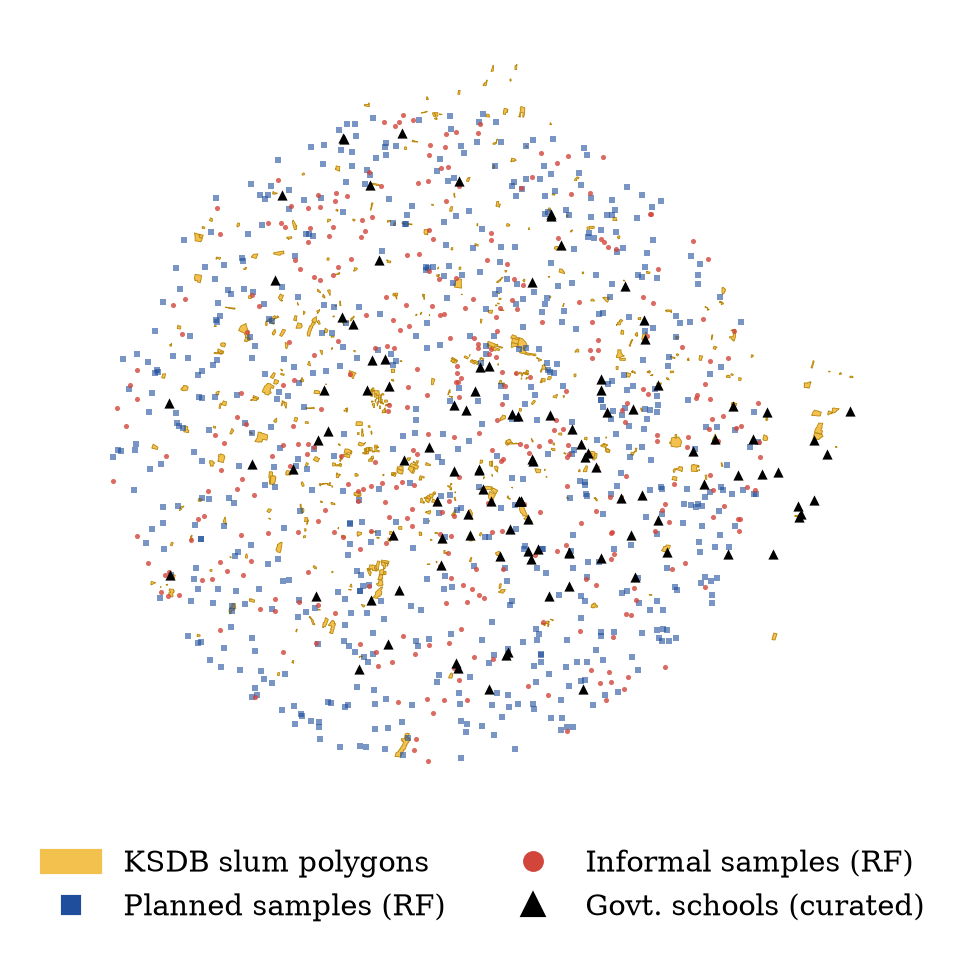
\includegraphics[width=0.82\columnwidth]{fig_study_area.png}
\caption{Study area. KSDB slum polygons (yellow), Random Forest sample locations classified as planned (blue squares) and informal (red circles) within the 15\km{} classification radius, and the 111 curated government schools (black triangles).}
\label{fig:study}
\end{figure}

Table~\ref{tab:data} lists the datasets, all of which are open or publicly released.

\begin{table}[!t]
\centering
\caption{Datasets Used}
\label{tab:data}
\footnotesize
\begin{tabularx}{\columnwidth}{@{}p{1.75cm}Xp{2.2cm}@{}}
\toprule
\textbf{Dataset} & \textbf{Content used} & \textbf{Size} \\
\midrule
Sentinel-2 L2A \cite{drusch2012} & Surface reflectance B4, B8, B11; Jan--Feb 2024 median composite, cloud $<5\%$ & 10\m{} raster \\
OSM walk network \cite{boeing2017} & Pedestrian-accessible ways, private access excluded & 186,595 nodes; 499,950 directed edges \\
OSM schools & \texttt{amenity=school} features with names & 1,464 features \\
KSDB slums & Slum polygons with zone and notification status & 509 polygons \\
WorldPop 2020 \cite{tatem2017} & 100\m{} population, summed per slum polygon & 226,753 residents \\
\bottomrule
\end{tabularx}
\end{table}

\subsection{School Data and the Government-School Definition}
OSM returned 1,464 school features (886 building or campus polygons and 578 points), of which 202 are unnamed. OSM ownership tags are sparse in Bengaluru, so government schools must be identified largely from names. The initial pipeline used a \emph{broad} filter: \texttt{operator:type} matching ``public'' or ``government'', or a name containing ``Govt'', ``Government'', ``BBMP'' or ``Public''. It selected 271 schools. Inspection showed that 150 of these carry no government keyword, and 125 matched only on ``Public''. In Indian usage this word is common in private school names, and several of the schools in the broad set are visibly private institutions.

We therefore define a \emph{curated} set of government schools. A school is included only if a government keyword (government, govt, BBMP, GHPS, GLPS, GHS, GULPS, KGBV, corporation or municipal) appears in the leading part of its name, i.e., not merely in an address suffix such as ``, BBMP Agara''. Colleges and pre-university institutions are excluded. The curated set contains 111 schools, 49 of which are explicitly named as primary schools. The curated set is used for all primary results; the broad set is reported for comparison with the original pipeline (Table~\ref{tab:schools}).

\begin{table}[!t]
\centering
\caption{Government-School Identification}
\label{tab:schools}
\footnotesize
\begin{tabular}{@{}lr@{}}
\toprule
\textbf{Stage} & \textbf{Count} \\
\midrule
All OSM \texttt{amenity=school} features & 1,464 \\
Broad filter (initial pipeline) & 271 \\
\quad of which matched only on ``Public'' & 125 \\
\quad of which carry any government keyword & 121 \\
\quad keyword only in address suffix (removed) & 3 \\
\quad colleges / pre-university (removed) & 7 \\
\textbf{Curated government schools} & \textbf{111} \\
\quad explicitly primary-named & 49 \\
Non-government schools (all others) & 1,353 \\
\bottomrule
\end{tabular}
\end{table}

%=====================================================================
\section{Proposed Methodology}\label{sec:method}
%=====================================================================
Fig.~\ref{fig:pipeline} shows the four-phase pipeline. The phases are described below.

\begin{figure*}[!t]
\centering
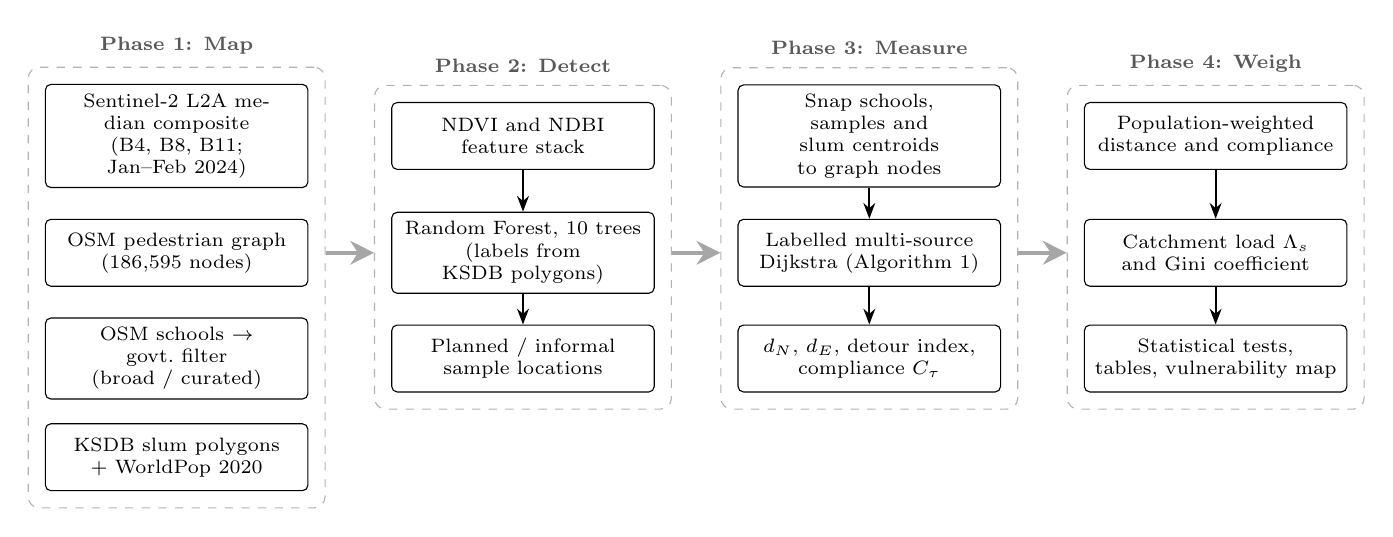
\begin{tikzpicture}[
  box/.style={draw, rounded corners=2pt, align=center, font=\scriptsize, minimum height=0.85cm, text width=3.1cm, fill=white},
  phase/.style={draw=gray!60, dashed, rounded corners=4pt, inner sep=6pt},
  lbl/.style={font=\scriptsize\bfseries, text=gray!70!black},
  arr/.style={-{Stealth[length=2mm]}, thick},
  big/.style={-{Stealth[length=3mm,width=3mm]}, line width=1.4pt, gray!70}]
\matrix[row sep=0.3cm, column sep=1.05cm] {
\node[box] (a1) {Sentinel-2 L2A median composite\\(B4, B8, B11; Jan--Feb 2024)}; &
\node[box] (b1) {NDVI and NDBI\\feature stack}; &
\node[box] (c1) {Snap schools, samples and\\slum centroids to graph nodes}; &
\node[box] (d1) {Population-weighted\\distance and compliance}; \\
\node[box] (a2) {OSM pedestrian graph\\(186,595 nodes)}; &
\node[box] (b2) {Random Forest, 10 trees\\(labels from KSDB polygons)}; &
\node[box] (c2) {Labelled multi-source\\Dijkstra (Algorithm 1)}; &
\node[box] (d2) {Catchment load $\Lambda_s$\\and Gini coefficient}; \\
\node[box] (a3) {OSM schools $\rightarrow$\\govt.\ filter (broad / curated)}; &
\node[box] (b3) {Planned / informal\\sample locations}; &
\node[box] (c3) {$d_N$, $d_E$, detour index,\\compliance $C_\tau$}; &
\node[box] (d3) {Statistical tests,\\tables, vulnerability map}; \\
\node[box] (a4) {KSDB slum polygons\\+ WorldPop 2020}; &
& & \\
};
\foreach \c in {b,c,d} {\draw[arr] (\c1) -- (\c2); \draw[arr] (\c2) -- (\c3);}
\node[phase, fit=(a1)(a4)] (p1) {};
\node[phase, fit=(b1)(b3)] (p2) {};
\node[phase, fit=(c1)(c3)] (p3) {};
\node[phase, fit=(d1)(d3)] (p4) {};
\node[lbl, above=1pt of p1] {Phase 1: Map};
\node[lbl, above=1pt of p2] {Phase 2: Detect};
\node[lbl, above=1pt of p3] {Phase 3: Measure};
\node[lbl, above=1pt of p4] {Phase 4: Weigh};
\draw[big] (p1.east |- b2) -- (p2.west |- b2);
\draw[big] (p2.east |- c2) -- (p3.west |- c2);
\draw[big] (p3.east |- d2) -- (p4.west |- d2);
\end{tikzpicture}
\caption{Proposed pipeline. Phase 1 ingests open data; Phase 2 classifies built-up morphology from Sentinel-2 (training labels drawn from KSDB polygons); Phase 3 computes network distances with a labelled multi-source Dijkstra search; Phase 4 weights results by population and derives catchment loads.}
\label{fig:pipeline}
\end{figure*}

\subsection{Phase 1: Data Acquisition and Pre-processing (Map)}
Three ingestion streams initialise the pipeline. (i) A Sentinel-2 surface-reflectance median composite is built in GEE from scenes acquired between 1 January and 1 March 2024 (the dry season) with less than 5\% cloudy pixels, clipped to the 15\km{} study radius. The median operator suppresses transient clouds and shadows. (ii) The pedestrian network is downloaded with OSMnx using \texttt{network\_type="walk"} and a custom filter that excludes area features and ways tagged \texttt{access=private}. The graph has 186,595 nodes and 499,950 directed edges, with a median edge length of 40.4\m{} (mean 61.0\m{}). (iii) School features are fetched with \texttt{features\_from\_place} for \texttt{amenity=school}. Polygon features are reduced to centroids computed in the projected UTM zone 43N coordinate system (EPSG:32643) and then converted back to WGS-84.

\subsection{Phase 2: Satellite Classification of Built-up Morphology (Detect)}
Two spectral indices are computed from the composite:
\begin{equation}
\mathrm{NDVI}=\frac{\rho_{\mathrm{NIR}}-\rho_{\mathrm{Red}}}{\rho_{\mathrm{NIR}}+\rho_{\mathrm{Red}}}=\frac{B8-B4}{B8+B4},
\end{equation}
\begin{equation}
\mathrm{NDBI}=\frac{\rho_{\mathrm{SWIR}}-\rho_{\mathrm{NIR}}}{\rho_{\mathrm{SWIR}}+\rho_{\mathrm{NIR}}}=\frac{B11-B8}{B11+B8}.
\end{equation}
NDVI \cite{tucker1979} suppresses vegetated pixels such as parks and tree-lined avenues; NDBI \cite{zha2003} emphasises impervious surfaces. The feature vector for each pixel is $\mathbf{x}=[B4, B8, B11, \mathrm{NDVI}, \mathrm{NDBI}]$.

Training data are drawn at 10\m{} scale. Class~1 (informal) consists of 2,000 pixels sampled inside KSDB slum polygons. Class~0 (planned) consists of 2,000 built-up pixels ($\mathrm{NDBI}>0$) sampled outside all slum polygons. A Random Forest \cite{breiman2001} with 10 trees is trained in GEE and applied to the full study area. Sample locations (``virtual students'') are then drawn at random from each predicted class; the exported sample files contain 364 informal and 636 planned locations.

\subsection{Phase 3: Network Accessibility (Measure)}
Let $G=(V,E,w)$ be the directed pedestrian graph with edge weights $w(e)$ equal to segment length in metres. Every origin $p$ (a sample location or slum centroid) and every school $s\in S$ is snapped to its nearest graph node, $v(p)$ and $v(s)$. The network distance from $p$ to the nearest government school is
\begin{equation}
d_N(p)=\min_{s\in S}\; \mathrm{dist}_G\big(v(p),v(s)\big),
\end{equation}
and the corresponding straight-line distance, computed in UTM coordinates, is
\begin{equation}
d_E(p)=\min_{s\in S}\; \lVert \mathbf{u}(p)-\mathbf{u}(s)\rVert_2 .
\end{equation}
Computing $d_N$ by running one shortest-path search per origin would be wasteful. Instead, we run a single multi-source Dijkstra search \cite{dijkstra1959} seeded simultaneously from all school nodes. Propagating the index of the seeding school as a \emph{label} alongside the tentative distance yields, on termination, both the distance to the nearest school and its identity at every node (Algorithm~1). This is the standard construction of the graph (network) Voronoi diagram \cite{erwig2000,okabe2008}; each Voronoi cell is the network catchment of one school. The search runs in $O\big((|V|+|E|)\log|V|\big)$ time; on the Bengaluru graph a full pass takes a few seconds on a laptop.

\begin{figure}[!t]
\hrule height 0.8pt\vspace{3pt}
\noindent\textbf{Algorithm 1:} Labelled multi-source Dijkstra\vspace{2pt}
\hrule\vspace{3pt}
{\footnotesize
\noindent\textbf{Input:} graph $G=(V,E,w)$; school nodes $s_1,\dots,s_k$\\
\textbf{Output:} distance $D[v]$ and nearest-school label $L[v]$ for all reachable $v$
\begin{enumerate}\setlength\itemsep{0pt}
\item $D[v]\leftarrow\infty$ for all $v\in V$; priority queue $Q\leftarrow\emptyset$
\item \textbf{for} $i=1$ \textbf{to} $k$: \textbf{if} $D[s_i]=\infty$: $D[s_i]\leftarrow0$; $L[s_i]\leftarrow i$; push $(0,s_i,i)$ to $Q$
\item \textbf{while} $Q\neq\emptyset$:
\item \quad pop $(d,u,i)$ with minimum $d$
\item \quad \textbf{if} $d>D[u]$: \textbf{continue} \hfill (stale entry)
\item \quad \textbf{for each} $(u,v)\in E$:
\item \quad\quad \textbf{if} $d+w(u,v)<D[v]$:
\item \quad\quad\quad $D[v]\leftarrow d+w(u,v)$; $L[v]\leftarrow i$; push $(D[v],v,i)$
\item \textbf{return} $D$, $L$
\end{enumerate}}
\vspace{-2pt}\hrule height 0.8pt
\end{figure}

The \emph{detour index} of an origin is $\eta(p)=d_N(p)/d_E(p)$ (with $d_E$ floored at 50\m{} to avoid division by near-zero distances). The RTE compliance rate of a set of origins $P$ at threshold $\tau$ is
\begin{equation}
C_\tau(P)=\frac{1}{|P|}\sum_{p\in P}\mathbf{1}\big[d_N(p)\le\tau\big],
\end{equation}
with $\tau=1{,}000\m{}$ for primary schooling. The crow-flies compliance rate $C^E_\tau$ is defined analogously with $d_E$. The \emph{false-compliance} share is the fraction of crow-flies-compliant origins that are not network-compliant.

\subsection{Phase 4: Population Weighting and Catchment Load (Weigh)}
For each KSDB slum $k$ with WorldPop population $\pi_k$, the population-weighted network distance and population compliance are
\begin{equation}
\bar d_\pi=\frac{\sum_k \pi_k\, d_N(c_k)}{\sum_k \pi_k},\qquad
C^\pi_\tau=\frac{\sum_k \pi_k\,\mathbf{1}[d_N(c_k)\le\tau]}{\sum_k \pi_k},
\end{equation}
where $c_k$ is the slum centroid. Using the labels from Algorithm~1, the \emph{catchment load} of school $s$ is the slum population for which $s$ is the nearest government school by network:
\begin{equation}
\Lambda_s=\sum_k \pi_k\,\mathbf{1}\big[L[v(c_k)]=s\big].
\end{equation}
Inequality of loads across schools is summarised with the Gini coefficient
\begin{equation}
\mathcal{G}=\frac{\sum_{i}\sum_{j}|\Lambda_i-\Lambda_j|}{2|S|^2\,\bar\Lambda}.
\end{equation}
Because school enrolment capacity is not available for Bengaluru in open form, $\Lambda_s$ measures the \emph{potential} demand that falls on each school, not its utilisation.

\subsection{Statistical Analysis}
Network distances are right-skewed, so formal and informal samples are compared with the two-sided Mann--Whitney $U$ test \cite{mann1947}. Effect size is reported as Cliff's $\delta$ \cite{cliff1993}, interpreted with the thresholds of Romano \textit{et al.}\ \cite{romano2006} ($|\delta|<0.147$ negligible, $<0.33$ small, $<0.474$ medium). The full distributions are compared with the two-sample Kolmogorov--Smirnov test. Compliance proportions are compared with a $\chi^2$ test. A 95\% confidence interval for the difference in means is obtained by the percentile bootstrap with 5,000 resamples \cite{efron1993}.

\subsection{Implementation}
Classification runs in GEE via \texttt{geemap}; routing and analysis use OSMnx 2.1, NetworkX, GeoPandas and SciPy. A single script, \texttt{scripts/paper\_analysis.py}, regenerates every number and figure in Section~\ref{sec:results} in about 20\,s.

%=====================================================================
\section{Results}\label{sec:results}
%=====================================================================
\subsection{Walking Distance from Classified Locations}
Table~\ref{tab:desc} summarises the network and straight-line distances from the 1,000 sample locations to the nearest curated government school. Distances are long in both zone types. The median planned location is 2.07\km{} from a government school by network and the median informal location is 1.92\km{}. Only 16.5\% of planned and 18.7\% of informal locations are within the 1\km{} RTE neighbourhood, and roughly half of each group is more than 2\km{} away.

\begin{table}[!t]
\centering
\caption{Distance to Nearest Government School (Curated Set, $n=111$ Schools)}
\label{tab:desc}
\footnotesize
\begin{threeparttable}
\begin{tabular}{@{}lrrrr@{}}
\toprule
& \multicolumn{2}{c}{\textbf{Network $d_N$ (m)}} & \multicolumn{2}{c}{\textbf{Straight line $d_E$ (m)}} \\
\cmidrule(lr){2-3}\cmidrule(l){4-5}
\textbf{Statistic} & \textbf{Planned} & \textbf{Informal} & \textbf{Planned} & \textbf{Informal} \\
\midrule
$n$ & 636 & 364 & 636 & 364 \\
Mean & 2,318 & 2,098 & 1,662 & 1,503 \\
Std.\ dev. & 1,557 & 1,164 & 1,041 & 913 \\
Median & 2,070 & 1,919 & 1,448 & 1,316 \\
Q1 -- Q3 & 1,239--3,024 & 1,244--2,884 & 848--2,245 & 813--1,982 \\
90th pct. & 4,207 & 3,677 & 3,231 & 2,764 \\
$\le$ 1\km{} (\%) & 16.5 & 18.7 & 31.8 & 35.2 \\
$>$ 2\km{} (\%) & 52.7 & 48.1 & 31.8 & 24.5 \\
Median detour $\eta$ & 1.35 & 1.35 & --- & --- \\
\bottomrule
\end{tabular}
\begin{tablenotes}\footnotesize
\item Median snapping distance: 37.6\m{} (planned), 47.0\m{} (informal), 28.8\m{} (schools).
\end{tablenotes}
\end{threeparttable}
\end{table}

\subsection{Formal versus Informal: How Large Is the Difference?}
Table~\ref{tab:tests} reports the statistical comparison. With curated schools, planned locations are on average 220\m{} farther than informal locations (95\% bootstrap CI: 41--382\m{}). However, the rank-based Mann--Whitney test is not significant at the 5\% level ($p=0.094$), the Kolmogorov--Smirnov test finds no difference in distributions ($p=0.18$), the compliance rates do not differ ($\chi^2$ $p=0.43$), and Cliff's $\delta=0.06$ is negligible. With the broad filter, the same direction appears more strongly ($p=0.004$, $\delta=0.11$), but that filter counts private schools as government schools.

The direction of the gap is consistent---planned layouts are, if anything, farther from government schools---but its magnitude is small compared with the distance both groups must walk. Relaxing the threshold to 3\km{}, the RTE norm for Classes VI--VIII, raises compliance to 74.4\% (planned) and 79.9\% (informal), so the shortfall falls hardest on the youngest children.

\begin{table}[!t]
\centering
\caption{Planned vs.\ Informal Comparison under Two Government-School Definitions}
\label{tab:tests}
\footnotesize
\begin{tabular}{@{}lrr@{}}
\toprule
\textbf{Quantity} & \textbf{Curated (111)} & \textbf{Broad (271)} \\
\midrule
Mean $d_N$, planned (m) & 2,318 & 1,548 \\
Mean $d_N$, informal (m) & 2,098 & 1,351 \\
Mean difference (m) & 220 & 197 \\
95\% bootstrap CI (m) & [41, 382] & [81, 314] \\
Mann--Whitney $U$ & 123,120 & 128,255 \\
\quad $p$-value & 0.094 & 0.004 \\
Cliff's $\delta$ & 0.06 (negl.) & 0.11 (negl.) \\
KS statistic $D$ ($p$) & 0.072 (0.18) & 0.091 (0.04) \\
$\chi^2$ on 1\km{} compliance ($p$) & 0.62 (0.43) & 5.47 (0.02) \\
Compliance $\le$1\km{}, planned (\%) & 16.5 & 32.5 \\
Compliance $\le$1\km{}, informal (\%) & 18.7 & 40.1 \\
\bottomrule
\end{tabular}
\end{table}

\subsection{The Crow-Flies Fallacy}\label{sec:crowflies}
Fig.~\ref{fig:euclid} plots network against straight-line distance for every sample location, and Table~\ref{tab:crow} summarises the effect on compliance. Network and Euclidean distances are strongly rank-correlated (Spearman $\rho=0.93$), but the median detour index is 1.35: a typical walk is roughly one-third longer than the straight line. At the 1\km{} threshold this matters a great deal. A straight-line audit would classify 33.0\% of locations as compliant, whereas the network audit finds 17.3\%. Of the locations that a crow-flies buffer would certify as compliant, 48.2\% are actually more than 1\km{} away on foot. With the broad school set the pattern is the same: 58.9\% vs.\ 35.3\%, a false-compliance share of 41.4\%.

\begin{figure}[!t]
\centering
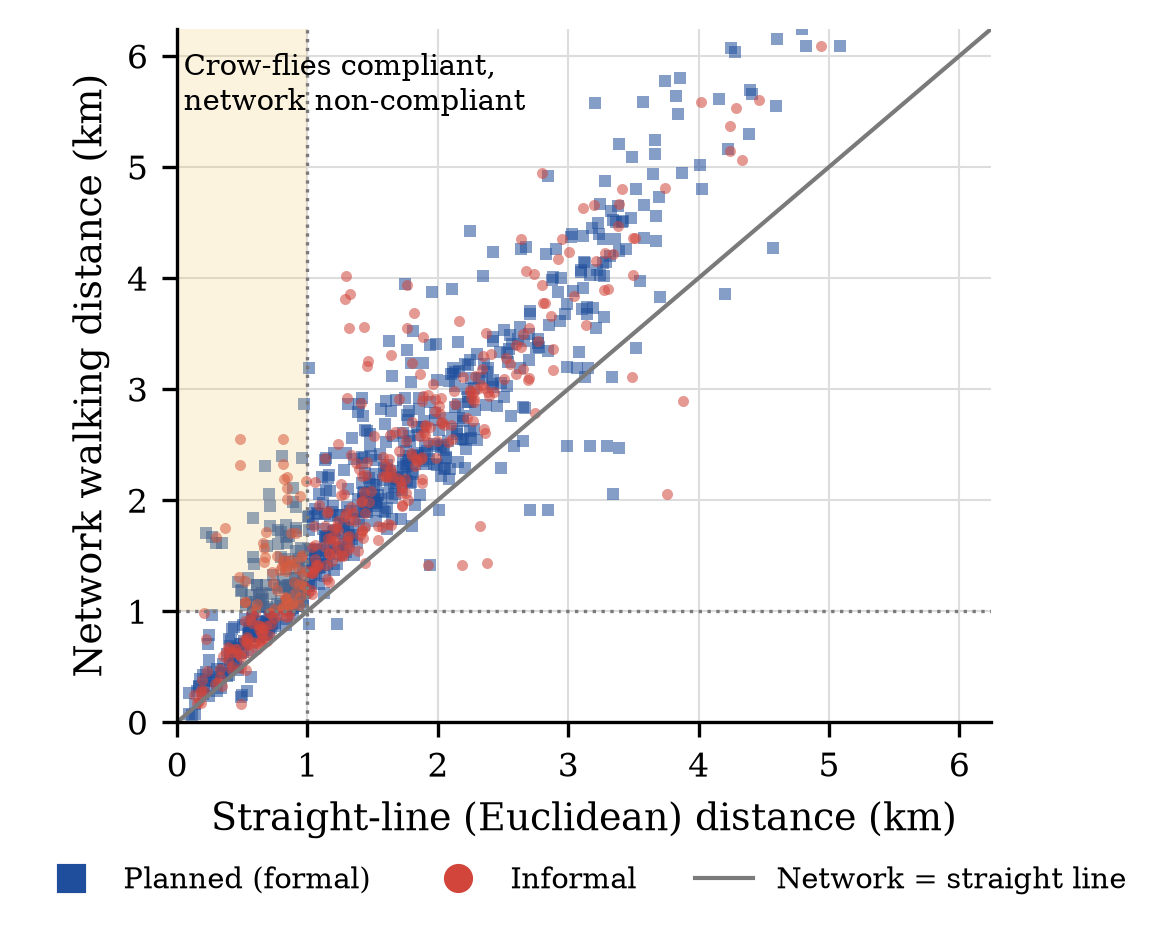
\includegraphics[width=\columnwidth]{fig_euclid_vs_network.png}
\caption{Network vs.\ straight-line distance to the nearest curated government school. Points in the shaded region lie within 1\km{} in a straight line but more than 1\km{} by the street network.}
\label{fig:euclid}
\end{figure}

\begin{table}[!t]
\centering
\caption{Straight-Line vs.\ Network Compliance at 1\km{}}
\label{tab:crow}
\footnotesize
\begin{tabular}{@{}lrr@{}}
\toprule
\textbf{Quantity} & \textbf{Curated} & \textbf{Broad} \\
\midrule
Crow-flies compliant, $C^E_{1\mathrm{km}}$ (\%) & 33.0 & 58.9 \\
Network compliant, $C_{1\mathrm{km}}$ (\%) & 17.3 & 35.3 \\
False-compliant, share of all locations (\%) & 15.9 & 24.4 \\
False-compliant, share of crow-flies compliant (\%) & 48.2 & 41.4 \\
Spearman $\rho(d_N,d_E)$ & 0.93 & 0.87 \\
\bottomrule
\end{tabular}
\end{table}

\subsection{Population-Weighted Access for KSDB Slums}\label{sec:slums}
The classified sample locations depend on the satellite classifier (see Section~\ref{sec:validity}). The KSDB slum polygons offer an independent, register-based view. Table~\ref{tab:slums} reports network access for all 509 polygons, which together hold an estimated 226,753 residents (median slum: 1.25\,ha, 127 residents, 187 residents/ha). With curated schools, the median slum centroid is 1.72\km{} from a government school by network. The population-weighted distance is 2.02\km{}, and only 20.1\% of slum residents live within the 1\km{} RTE neighbourhood. 39.1\% of slums are more than 2\km{} away.

\begin{table}[!t]
\centering
\caption{Network Access for KSDB Slums (WorldPop-Weighted)}
\label{tab:slums}
\footnotesize
\begin{tabular}{@{}lrr@{}}
\toprule
\textbf{Quantity} & \textbf{Curated} & \textbf{Broad} \\
\midrule
Slums routed & 509 & 509 \\
Residents (WorldPop 2020) & 226,753 & 226,753 \\
Median slum distance (m) & 1,723 & 1,103 \\
Population-weighted distance (m) & 2,023 & 1,331 \\
Slums within 1\km{} (\%) & 27.7 & 45.8 \\
Residents within 1\km{} (\%) & 20.1 & 39.2 \\
Slums beyond 2\km{} (\%) & 39.1 & 11.6 \\
Spearman $\rho$(population, distance) & 0.06 ($p$=0.15) & 0.05 ($p$=0.28) \\
\bottomrule
\end{tabular}
\end{table}

Fig.~\ref{fig:slumpop} plots each slum's distance against its population. There is no relationship between settlement size and distance ($\rho=0.06$, $p=0.15$), nor between density and distance ($\rho=-0.02$, $p=0.59$). Large slums are no better served than small ones.

\begin{figure}[!t]
\centering
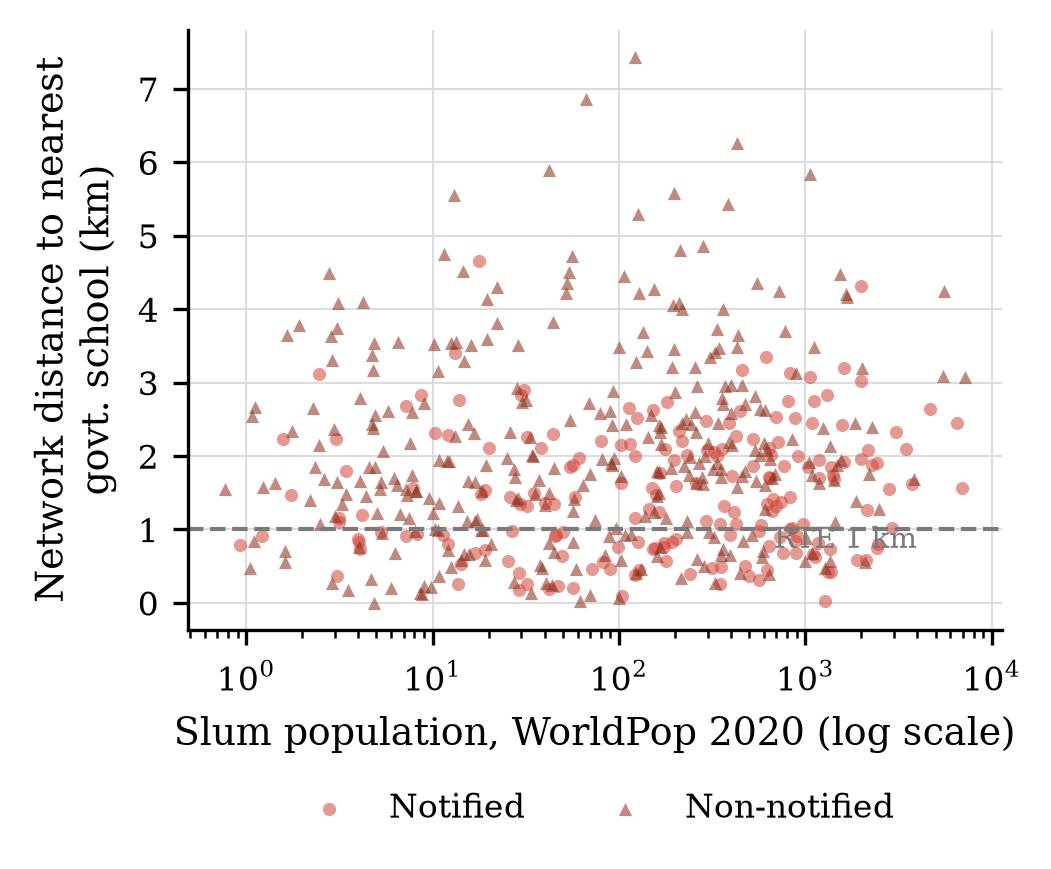
\includegraphics[width=\columnwidth]{fig_slum_pop_vs_distance.png}
\caption{Network distance to the nearest curated government school vs.\ WorldPop population for each KSDB slum, by notification status. Settlement size does not predict proximity.}
\label{fig:slumpop}
\end{figure}

\subsubsection{Notified versus non-notified slums}
Table~\ref{tab:notif} separates slums by notification status. Non-notified slums, i.e., settlements on the register but without legal notification, are significantly farther from government schools than notified ones. The population-weighted distance is 2.40 vs.\ 1.71\km{}, and only 15.5\% of non-notified residents are within 1\km{}, compared with 24.0\% of notified residents (Mann--Whitney $p=1.5\times10^{-6}$, Cliff's $\delta=0.25$, small). The difference persists with the broad school set ($p=0.002$, $\delta=0.16$).

\begin{table}[!t]
\centering
\caption{Access by Slum Notification Status (Curated Schools)}
\label{tab:notif}
\footnotesize
\begin{tabular}{@{}lrr@{}}
\toprule
\textbf{Quantity} & \textbf{Notified} & \textbf{Non-notified} \\
\midrule
Slums & 192 & 317 \\
Residents & 122,705 & 104,049 \\
Median distance (m) & 1,441 & 1,862 \\
Population-weighted distance (m) & 1,707 & 2,396 \\
Slums within 1\km{} (\%) & 35.9 & 22.7 \\
Residents within 1\km{} (\%) & 24.0 & 15.5 \\
\bottomrule
\end{tabular}
\end{table}

\subsubsection{Administrative zones}
Access varies sharply between the city's administrative zones (Table~\ref{tab:zones}). South zone is best served: 43.8\% of its slum residents are within 1\km{}, at a population-weighted distance of 1.17\km{}. Dasarahalli, Yelahanka and Bommanahalli are the worst: population-weighted distances exceed 3\km{}, and in Dasarahalli fewer than 1\% of slum residents are within 1\km{} of a curated government school. The peripheral zones, where much post-2011 growth has occurred, are the least served.

\begin{table}[!t]
\centering
\caption{Slum Access by Administrative Zone (Curated Schools)}
\label{tab:zones}
\footnotesize
\begin{tabular}{@{}lrrrr@{}}
\toprule
\textbf{Zone} & \textbf{Slums} & \textbf{Residents} & \textbf{Pop.-wtd.} & \textbf{Res.\ $\le$1\km{}} \\
 & & & \textbf{dist.\ (m)} & \textbf{(\%)} \\
\midrule
South & 93 & 48,486 & 1,167 & 43.8 \\
Mahadevapura & 90 & 1,366 & 1,507 & 35.8 \\
West & 90 & 67,150 & 1,889 & 17.9 \\
East & 103 & 54,730 & 2,079 & 17.6 \\
RR Nagar & 55 & 24,690 & 2,443 & 4.4 \\
Yelahanka & 46 & 11,101 & 3,170 & 8.6 \\
Bommanahalli & 14 & 325 & 3,174 & 10.1 \\
Dasarahalli & 18 & 18,906 & 3,330 & 0.7 \\
\bottomrule
\end{tabular}
\end{table}

\subsection{Catchment Load: Where Slum Demand Falls}
Algorithm~1 assigns every slum to its nearest government school. Of the 111 curated schools, 81 are the nearest school for at least one slum, and 30 serve none. The distribution of potential demand is extremely unequal (Table~\ref{tab:load}). The median school with a slum catchment receives 179 slum residents, the mean is 2,799, and the most-loaded school receives 28,193. The ten most-loaded schools are the nearest government option for 71.5\% of all slum residents, and the Gini coefficient of loads is 0.85. With the broad filter the Gini is similar (0.87), but the most-loaded ``government'' schools are private institutions with ``Public'' in their names.

\begin{table}[!t]
\centering
\caption{Most-Loaded Government Schools (Curated Set)}
\label{tab:load}
\footnotesize
\begin{tabularx}{\columnwidth}{@{}Xrr@{}}
\toprule
\textbf{School (OSM name)} & \textbf{Slums} & \textbf{Residents} \\
\midrule
Haji Sir Ismail Sait Govt.\ Urdu \& English HPS & 25 & 28,193 \\
Nammura Government Model Primary School & 22 & 26,242 \\
Government School (generic OSM name) & 27 & 23,453 \\
Gangamma Thimmaiah Govt.\ School & 14 & 16,339 \\
Jindal Government School & 10 & 16,223 \\
\midrule
Top-10 share of slum residents & \multicolumn{2}{r}{71.5\%} \\
Gini coefficient of loads & \multicolumn{2}{r}{0.85} \\
\bottomrule
\end{tabularx}
\end{table}

\subsection{Proximity to Non-Government Schools}
The 1,353 OSM school features outside the curated government set are much closer to every location (Table~\ref{tab:private}). The median planned location is 0.69\km{} from a non-government school and the median informal location 0.60\km{}; 71.2\% and 76.4\% respectively are within 1\km{}. The open data therefore describe a city in which a school of \emph{some} kind is usually within walking distance, but a free government school usually is not.

\begin{table}[!t]
\centering
\caption{Network Distance to Nearest Government vs.\ Non-Government School}
\label{tab:private}
\footnotesize
\begin{tabular}{@{}lrrrr@{}}
\toprule
& \multicolumn{2}{c}{\textbf{Govt.\ (curated)}} & \multicolumn{2}{c}{\textbf{Non-govt.}} \\
\cmidrule(lr){2-3}\cmidrule(l){4-5}
& \textbf{Plan.} & \textbf{Inf.} & \textbf{Plan.} & \textbf{Inf.} \\
\midrule
Median (m) & 2,070 & 1,919 & 691 & 598 \\
Mean (m) & 2,318 & 2,098 & 858 & 757 \\
$\le$ 1\km{} (\%) & 16.5 & 18.7 & 71.2 & 76.4 \\
$>$ 2\km{} (\%) & 52.7 & 48.1 & 5.3 & 4.7 \\
\bottomrule
\end{tabular}
\end{table}

\subsection{Vulnerability Map}
Fig.~\ref{fig:vmap} maps compliance across the city using the curated government schools: (a) the classified sample locations and (b) the KSDB slums, each coloured by network walking distance. Non-compliant locations dominate the periphery, and the large slums in the West and RR~Nagar zones form the most extensive cluster beyond 2\km{}. The pipeline also exports the same layers as an interactive web map (Leaflet via \texttt{folium}), in which each marker's pop-up reports its zone, population and walking distance.

\begin{figure*}[!t]
\centering
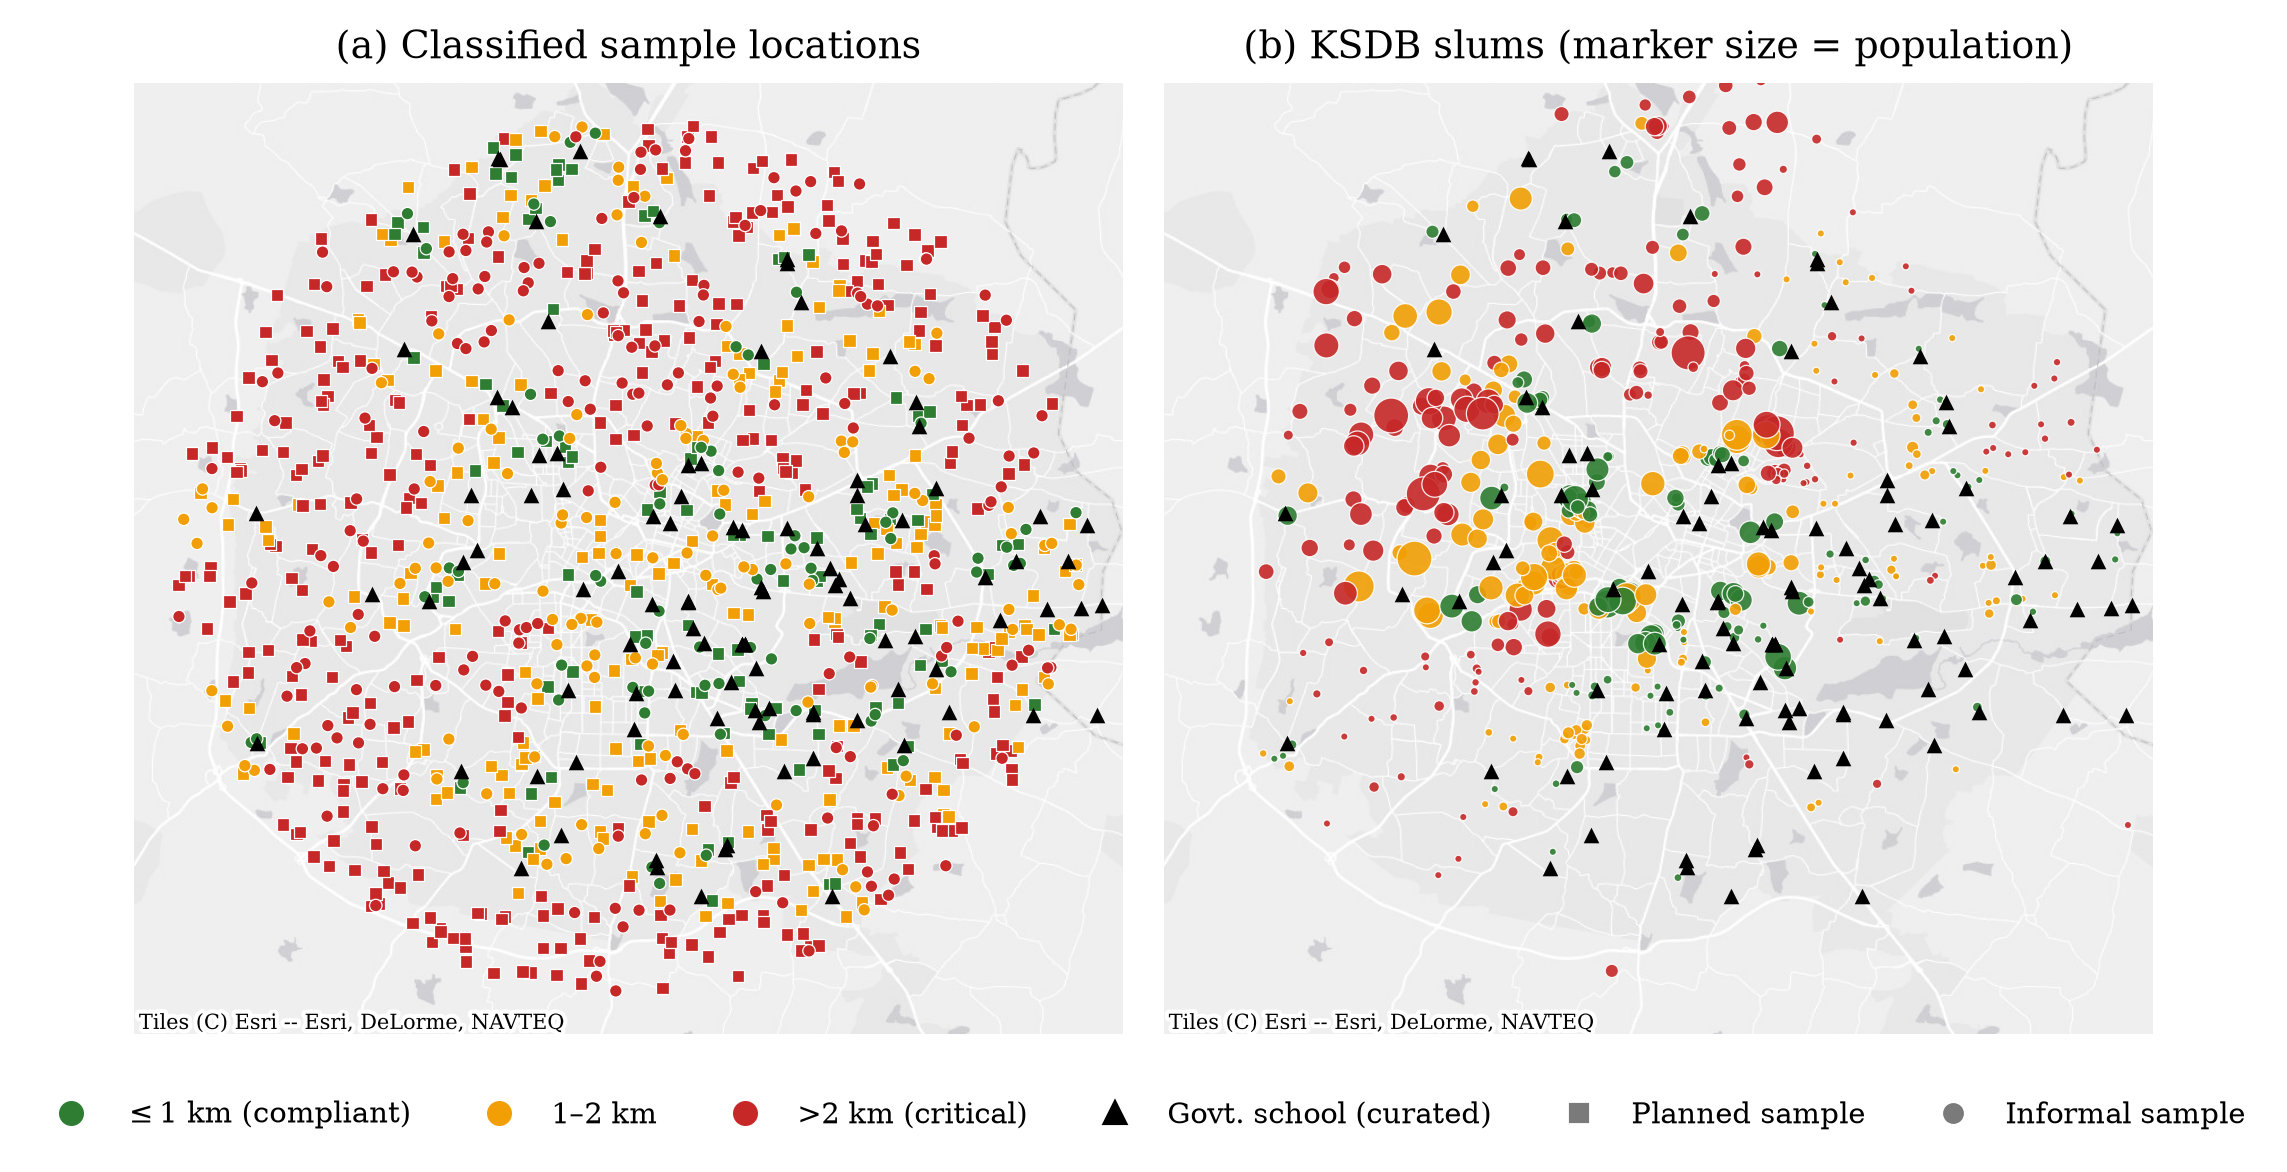
\includegraphics[width=\textwidth]{fig_vulnerability_map.png}
\caption{Vulnerability map of Bengaluru (curated government schools). Colour gives network walking distance to the nearest government school: green $\le$1\km{} (compliant), orange 1--2\km{}, red $>$2\km{} (critical). (a) Random Forest sample locations (squares: planned; circles: informal). (b) KSDB slum centroids, sized by WorldPop population. Black triangles are curated government schools.}
\label{fig:vmap}
\end{figure*}

%=====================================================================
\section{Discussion}\label{sec:discussion}
%=====================================================================
\subsection{A City-Wide Gap that Falls on the Invisible}
The most robust finding does not depend on the formal--informal distinction: most locations and most slum residents in Bengaluru cannot reach a government school within the 1\km{} walk the RTE rules promise, under both school definitions. The clearest equity signal concerns administrative visibility: non-notified slums and peripheral zones are the least served, and these are exactly the settlements least likely to appear in the planning frames used by conventional audits.

\subsection{Privatised Substitution}
Planned layouts are slightly farther from government schools than informal areas and lie close to dense networks of non-government schools, consistent with demand shifting to private schools where households can pay \cite{kingdon2020}. Karnataka policy raises the stakes of this geometry. A January 2019 amendment to Rule~4 of the Karnataka RTE Rules exempted private unaided schools from the 25\% RTE quota in neighbourhoods that have a government or aided school, and was upheld by the Karnataka High Court in May 2019 \cite{hc2019}; RTE-quota admissions have since been reported to have fallen from over one lakh in 2018 to 3,412 \cite{tnie2026}. Whether a government school is ``in the neighbourhood'' now decides whether a poor child can claim a free private seat, so the walking-distance audit has direct consequences. Our data cannot establish causality, and the hypothesis that planned layouts are strongly disadvantaged is not supported once private schools are removed from the government set.

\subsection{From Distance to Load}
Settlement population and density do not predict distance, but potential slum demand is concentrated on a few schools. Without open capacity data we cannot say whether these schools are overcrowded; the load ranking nevertheless gives planners a short list of schools to check first and can feed capacity-aware 2SFCA \cite{luo2003} once capacities are known. For auditing practice, three recommendations follow: use network rather than straight-line distance, include the full slum register rather than notified slums only, and curate the identity of ``government schools'' in open data.

%=====================================================================
\section{Threats to Validity and Limitations}\label{sec:validity}
%=====================================================================
\subsection{Agreement between the Classifier and KSDB Ground Truth}
The Random Forest was trained on pixels inside KSDB polygons, yet its predicted classes agree poorly with those polygons at the sample locations (Table~\ref{tab:agree}). Only 1.9\% of locations predicted informal fall inside a KSDB polygon (vs.\ 0.8\% of planned locations), and within 250\m{} or 500\m{} buffers the two classes are indistinguishable. Several factors contribute. KSDB slums are small (median 1.25\,ha, i.e., about 125 Sentinel-2 pixels), so at 10\m{} resolution many slum pixels are spectrally mixed with their surroundings, as Wurm \textit{et al.}\ \cite{wurm2019} also found. The KSDB register is also incomplete, and the model uses only five spectral features with no texture. Formal accuracy assessment on held-out labelled data was not performed. Consequently, the ``informal'' class should be read as \emph{informal-like spectral morphology}, not as verified slum. This is why we report the KSDB-based results (Section~\ref{sec:slums}) alongside the classified-sample results, and why our equity conclusions rest primarily on the former.

\begin{table}[!t]
\centering
\caption{Agreement of Classified Samples with KSDB Slum Polygons}
\label{tab:agree}
\footnotesize
\begin{tabular}{@{}lrr@{}}
\toprule
\textbf{Share of samples (\%)} & \textbf{Pred.\ informal} & \textbf{Pred.\ planned} \\
\midrule
Inside a KSDB polygon & 1.9 & 0.8 \\
Within 100\m{} of a polygon & 6.9 & 6.1 \\
Within 250\m{} of a polygon & 15.9 & 16.4 \\
Within 500\m{} of a polygon & 41.2 & 39.6 \\
\midrule
$n$ & 364 & 636 \\
\bottomrule
\end{tabular}
\end{table}

\subsection{Data and Modelling Assumptions}
OSM under-records government schools, and those that are unmapped or unnamed are missing from both school sets; distances are therefore biased upward, and our compliance figures are best read as lower bounds on access. The curated filter trades recall for precision, so the broad and curated results bracket the plausible range; only 49 of the 111 curated schools are explicitly primary. Official UDISE+ records would remove this uncertainty, but they could not be used to validate OSM coverage: the public UDISE+ dashboard and reports (e.g., Report~1003, schools by management and category) are disaggregated only to state level for 2025--26, reporting 74,578 schools in Karnataka of which 65.07\% are government-managed, with no district- or city-level breakdown \cite{udise2026}, and school coordinates are available only to authorised users of the UDISE+ GIS portal. The completeness of OSM's government-school layer for Bengaluru therefore cannot be quantified from open data. Distances are measured node to node (median snapping leg 22--47\m{}), polygon schools are represented by centroids, and the network may omit informal footpaths (overstating distance) while ignoring crossing difficulty (understating it). WorldPop is modelled and uncertain in dense informal areas, and catchment loads count all residents rather than school-age children.

%=====================================================================
\section{Conclusion and Future Work}\label{sec:conclusion}
%=====================================================================
This paper presented an open, reproducible pipeline for auditing the RTE walking-distance mandate. It combines Sentinel-2 classification, OSM network routing with a labelled multi-source Dijkstra search, the KSDB slum register, and WorldPop population. Applied to Bengaluru, it shows that the compliance gap is city-wide: with curated government schools, only 17.3\% of sampled locations and 20.1\% of slum residents are within a 1\km{} walk. Planned layouts are marginally farther from government schools than informal areas, but the difference is negligible in effect size and sensitive to how government schools are identified. Straight-line audits overstate compliance, with nearly half of apparently compliant locations failing on the street network. Non-notified slums and peripheral zones are the least served, and potential slum demand concentrates on a handful of government schools.

\textbf{Future work} will address the limitations above:
\begin{enumerate}
\item \textbf{Authoritative school data.} Replace name-based filtering with UDISE+ school locations, management type and level (obtained through authorised access to the UDISE+ GIS portal), and add enrolment capacities to compute capacity-aware 2SFCA accessibility.
\item \textbf{Validated classification.} Add GLCM texture \cite{haralick1973} and VHR imagery, create an independent labelled validation set, and report a proper ablation with accuracy, precision, recall and F1-score.
\item \textbf{School-age population.} Use age-structured WorldPop layers to weight by children aged 6--14 rather than all residents.
\item \textbf{Public transit.} Integrate BMTC bus stops and routes to assess whether locations beyond walking range have viable transit access to schools.
\item \textbf{Siting optimisation and dashboard.} Deploy the pipeline as an interactive planning dashboard and add location--allocation optimisation to recommend sites for new government schools that maximise population-weighted 1\km{} coverage under budget constraints.
\end{enumerate}

\section*{Acknowledgement}
The authors gratefully acknowledge PES University, Bengaluru. We thank the European Space Agency for Sentinel-2 imagery, the OpenStreetMap contributors, the WorldPop project, and the Karnataka Slum Development Board for the slum register.

\begin{thebibliography}{00}
\bibitem{census2011} Office of the Registrar General \& Census Commissioner, India, ``Census of India 2011: Provisional population totals,'' Ministry of Home Affairs, Government of India, 2011.
\bibitem{unhabitat2003} UN-Habitat, \textit{The Challenge of Slums: Global Report on Human Settlements 2003}. London, U.K.: Earthscan, 2003.
\bibitem{rte2009} Government of India, ``The Right of Children to Free and Compulsory Education Act, 2009,'' \textit{The Gazette of India}, Act No.~35 of 2009.
\bibitem{rterules2010} Ministry of Human Resource Development, Government of India, ``The Right of Children to Free and Compulsory Education Rules, 2010,'' Rule~6, 2010. [Online]. Available: \url{https://indiankanoon.org/doc/42884596/} (accessed Oct. 5, 2026).
\bibitem{drusch2012} M. Drusch \textit{et al.}, ``Sentinel-2: ESA's optical high-resolution mission for GMES operational services,'' \textit{Remote Sens. Environ.}, vol.~120, pp.~25--36, 2012.
\bibitem{gorelick2017} N. Gorelick, M. Hancher, M. Dixon, S. Ilyushchenko, D. Thau, and R. Moore, ``Google Earth Engine: Planetary-scale geospatial analysis for everyone,'' \textit{Remote Sens. Environ.}, vol.~202, pp.~18--27, 2017.
\bibitem{boeing2017} G. Boeing, ``OSMnx: New methods for acquiring, constructing, analyzing, and visualizing complex street networks,'' \textit{Comput., Environ. Urban Syst.}, vol.~65, pp.~126--139, 2017, doi: 10.1016/j.compenvurbsys.2017.05.004.
\bibitem{tatem2017} A. J. Tatem, ``WorldPop, open data for spatial demography,'' \textit{Sci. Data}, vol.~4, Art.~no.~170004, 2017, doi: 10.1038/sdata.2017.4.
\bibitem{kuffer2016} M. Kuffer, K. Pfeffer, and R. Sliuzas, ``Slums from space---15 years of slum mapping using remote sensing,'' \textit{Remote Sens.}, vol.~8, no.~6, p.~455, 2016, doi: 10.3390/rs8060455.
\bibitem{kohli2012} D. Kohli, R. Sliuzas, N. Kerle, and A. Stein, ``An ontology of slums for image-based classification,'' \textit{Comput., Environ. Urban Syst.}, vol.~36, no.~2, pp.~154--163, 2012, doi: 10.1016/j.compenvurbsys.2011.11.001.
\bibitem{mahabir2018} R. Mahabir, A. Croitoru, A. T. Crooks, P. Agouris, and A. Stefanidis, ``A critical review of high and very high-resolution remote sensing approaches for detecting and mapping slums: Trends, challenges and emerging opportunities,'' \textit{Urban Sci.}, vol.~2, no.~1, p.~8, 2018, doi: 10.3390/urbansci2010008.
\bibitem{duque2015} J. C. Duque, J. E. Patino, L. A. Ruiz, and J. E. Pardo-Pascual, ``Measuring intra-urban poverty using land cover and texture metrics derived from remote sensing data,'' \textit{Landsc. Urban Plan.}, vol.~135, pp.~11--21, 2015.
\bibitem{haralick1973} R. M. Haralick, K. Shanmugam, and I. Dinstein, ``Textural features for image classification,'' \textit{IEEE Trans. Syst., Man, Cybern.}, vol.~SMC-3, no.~6, pp.~610--621, 1973.
\bibitem{wurm2019} M. Wurm, T. Stark, X. X. Zhu, M. Weigand, and H. Taubenb\"{o}ck, ``Semantic segmentation of slums in satellite images using transfer learning on fully convolutional neural networks,'' \textit{ISPRS J. Photogramm. Remote Sens.}, vol.~150, pp.~59--69, 2019, doi: 10.1016/j.isprsjprs.2019.02.006.
\bibitem{breiman2001} L. Breiman, ``Random forests,'' \textit{Mach. Learn.}, vol.~45, no.~1, pp.~5--32, 2001.
\bibitem{belgiu2016} M. Belgiu and L. Dr\u{a}gu\c{t}, ``Random forest in remote sensing: A review of applications and future directions,'' \textit{ISPRS J. Photogramm. Remote Sens.}, vol.~114, pp.~24--31, 2016.
\bibitem{tucker1979} C. J. Tucker, ``Red and photographic infrared linear combinations for monitoring vegetation,'' \textit{Remote Sens. Environ.}, vol.~8, no.~2, pp.~127--150, 1979.
\bibitem{zha2003} Y. Zha, J. Gao, and S. Ni, ``Use of normalized difference built-up index in automatically mapping urban areas from TM imagery,'' \textit{Int. J. Remote Sens.}, vol.~24, no.~3, pp.~583--594, 2003, doi: 10.1080/01431160304987.
\bibitem{talen1998} E. Talen and L. Anselin, ``Assessing spatial equity: An evaluation of measures of accessibility to public playgrounds,'' \textit{Environ. Plan. A}, vol.~30, no.~4, pp.~595--613, 1998, doi: 10.1068/a300595.
\bibitem{luo2003} W. Luo and F. Wang, ``Measures of spatial accessibility to health care in a GIS environment: Synthesis and a case study in the Chicago region,'' \textit{Environ. Plan. B}, vol.~30, no.~6, pp.~865--884, 2003, doi: 10.1068/b29120.
\bibitem{radke2000} J. Radke and L. Mu, ``Spatial decompositions, modeling and mapping service regions to predict access to social programs,'' \textit{Geogr. Inf. Sci.}, vol.~6, no.~2, pp.~105--112, 2000, doi: 10.1080/10824000009480538.
\bibitem{hagberg2008} A. A. Hagberg, D. A. Schult, and P. J. Swart, ``Exploring network structure, dynamics, and function using NetworkX,'' in \textit{Proc. 7th Python Sci. Conf. (SciPy)}, 2008, pp.~11--15.
\bibitem{erwig2000} M. Erwig, ``The graph Voronoi diagram with applications,'' \textit{Networks}, vol.~36, no.~3, pp.~156--163, 2000.
\bibitem{okabe2008} A. Okabe, T. Satoh, T. Furuta, A. Suzuki, and K. Okano, ``Generalized network Voronoi diagrams: Concepts, computational methods, and applications,'' \textit{Int. J. Geogr. Inf. Sci.}, vol.~22, no.~9, pp.~965--994, 2008.
\bibitem{dijkstra1959} E. W. Dijkstra, ``A note on two problems in connexion with graphs,'' \textit{Numer. Math.}, vol.~1, pp.~269--271, 1959.
\bibitem{haklay2010} M. Haklay, ``How good is volunteered geographical information? A comparative study of OpenStreetMap and Ordnance Survey datasets,'' \textit{Environ. Plan. B}, vol.~37, no.~4, pp.~682--703, 2010, doi: 10.1068/b35097.
\bibitem{barrington2017} C. Barrington-Leigh and A. Millard-Ball, ``The world's user-generated road map is more than 80\% complete,'' \textit{PLoS ONE}, vol.~12, no.~8, Art.~no.~e0180698, 2017, doi: 10.1371/journal.pone.0180698.
\bibitem{kingdon2020} G. G. Kingdon, ``The private schooling phenomenon in India: A review,'' \textit{J. Dev. Stud.}, vol.~56, no.~10, pp.~1795--1817, 2020, doi: 10.1080/00220388.2020.1715943.
\bibitem{muralidharan2015} K. Muralidharan and V. Sundararaman, ``The aggregate effect of school choice: Evidence from a two-stage experiment in India,'' \textit{Q. J. Econ.}, vol.~130, no.~3, pp.~1011--1066, 2015.
\bibitem{mann1947} H. B. Mann and D. R. Whitney, ``On a test of whether one of two random variables is stochastically larger than the other,'' \textit{Ann. Math. Statist.}, vol.~18, no.~1, pp.~50--60, 1947.
\bibitem{cliff1993} N. Cliff, ``Dominance statistics: Ordinal analyses to answer ordinal questions,'' \textit{Psychol. Bull.}, vol.~114, no.~3, pp.~494--509, 1993.
\bibitem{romano2006} J. Romano, J. D. Kromrey, J. Coraggio, and J. Skowronek, ``Appropriate statistics for ordinal level data: Should we really be using t-test and Cohen's d for evaluating group differences on the NSSE and other surveys?'' in \textit{Annu. Meeting Florida Assoc. Institutional Res.}, 2006.
\bibitem{efron1993} B. Efron and R. J. Tibshirani, \textit{An Introduction to the Bootstrap}. New York, NY, USA: Chapman \& Hall, 1993.
\bibitem{udise2026} Ministry of Education, Government of India, ``UDISE+ dashboard and Report 1003: Number of schools by school management and school category, Karnataka, 2025--26.'' [Online]. Available: \url{https://dashboard.udiseplus.gov.in} (accessed Oct. 5, 2026).
\bibitem{hc2019} High Court of Karnataka, \textit{Education Rights Trust v. Government of Karnataka}, judgment of May 31, 2019. [Online]. Available: \url{https://indiankanoon.org/doc/143950994/} (accessed Oct. 5, 2026).
\bibitem{tnie2026} The New Indian Express, ``Karnataka RTE intake plunges; panel calls for age expansion,'' Feb. 21, 2026. [Online]. Available: \url{https://www.newindianexpress.com/states/karnataka/2026/Feb/21/karnataka-rte-intake-plunges-panel-calls-for-age-expansion} (accessed Oct. 5, 2026).
\end{thebibliography}

\end{document}
